\subsection{Gang of four}

% Sensitivity function
\subsubsection{Sensitivity function}
$$
S(s) = \dfrac{1}{1 + PC}
$$
The Bode plots of the sensitivity function are given at figure \ref{fig:sensitivity}. That function tells us how the noise acts on the output. We do not want the system to react to the noise, as it is actually the measurement noise that must stay in the output.\par
That noise is a high-frequency phenomenon and, as can be seen on the Bode plots, there is no attenuation for high frequency, which is what we want.
\begin{figure}[H]
    \centering
    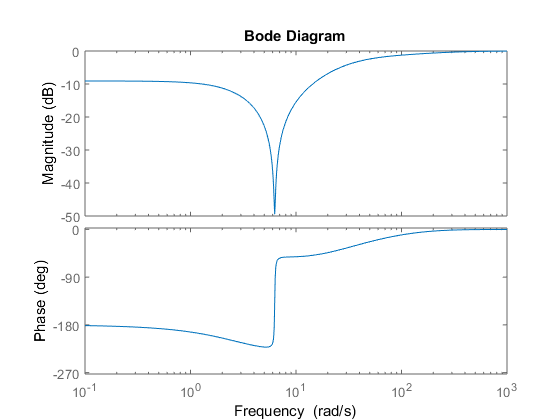
\includegraphics[width=0.8\textwidth]{resources/png/sensitivity.png}
    \caption{Bode plots of the sensitivity function}
    \label{fig:sensitivity}
\end{figure}

% Load sensitivity function
\subsubsection{Load sensitivity function}
$$
PS(s) = \dfrac{P}{1 + PC}
$$
This function tells us how the disturbances act on the output and the Bode diagrams are given at figure \ref{fig:load}. Our system needs to be robust against disturbances. In our case, these disturbances are low frequency phenomena (frequency of the wind, which we have either chosen constant or a sine function of frequency equal to 1). We can see that we have a very good reaction concerning the effect of the wind on the output of the system (attenuation of more than \SI{-200}{\deci\bel}).
\begin{figure}[H]
    \centering
    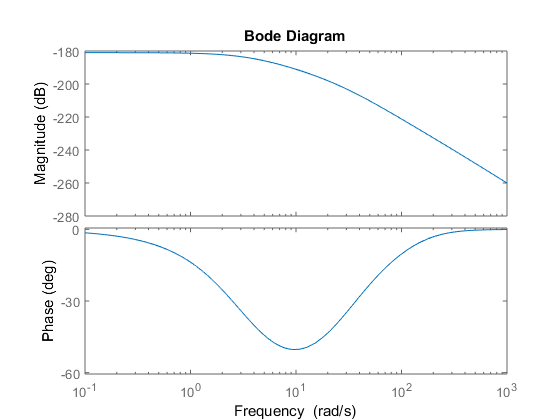
\includegraphics[width=0.8\textwidth]{resources/png/load.png}
    \caption{Bode plots of the load sensitivity function}
    \label{fig:load}
\end{figure}

% Complementary sensitivity function
\subsubsection{Complementary sensitivity function}
$$
PS(s) = \dfrac{PC}{1 + PC}
$$
This function tells us how the disturbances act on the controllable input and the reference acts on the output, and the Bode diagrams are given at figure \ref{fig:complementary-sensitivity}.\par
The control signal must be reactive to disturbance and the output should be able to track the reference. Amplitudes at low frequency should therefore not be dampened, and we see that they are not attenuated on the plots.
\begin{figure}[H]
    \centering
    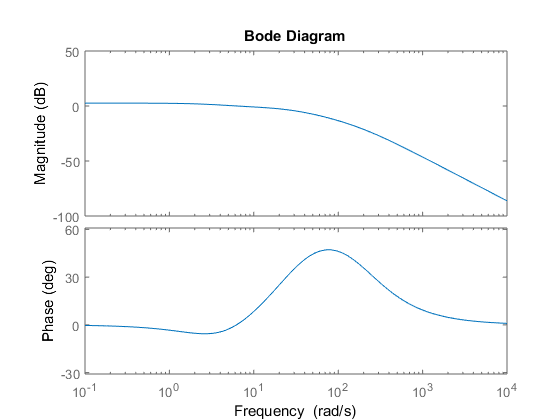
\includegraphics[width=0.8\textwidth]{resources/png/complementary-sensitivity.png}
    \caption{Bode plots of the complementary sensitivity function}
    \label{fig:complementary-sensitivity}
\end{figure}

% Noise sensitivity function
\subsubsection{Noise sensitivity function}
$$
PS(s) = \dfrac{C}{1 + PC}
$$
This function tells us how the noise and the reference act on the controllable input, and the Bode diagrams are given at figure \ref{fig:noise-sensitivity}.\par
That function should be reactive to reference changes, but not to noise, and so have a high magnitude at low frequency and low magnitude at high frequencies. We can see that it is not the case here. Indeed, we have high amplitudes for high frequencies. However, as our reference does not change in our system (we do not plan on dampening the oscillations in a Pisa Tower), it does not really matter.\par
It is also known that temporal domain controllers are better at reacting to reference changes than frequency domain ones.
\begin{figure}[H]
    \centering
    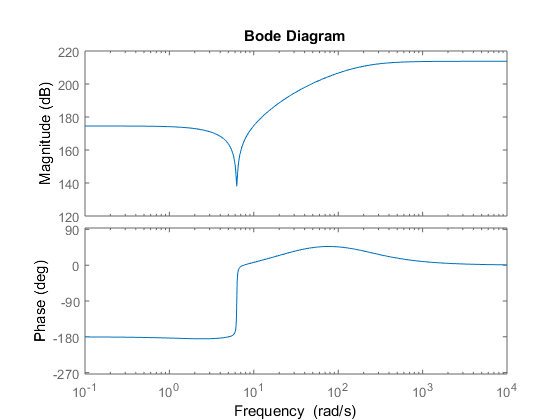
\includegraphics[width=0.8\textwidth]{resources/png/noise-sensitivity.png}
    \caption{Bode plots of the noise sensitivity function}
    \label{fig:noise-sensitivity}
\end{figure}
